\documentclass[a4paper,12pt]{article}

\usepackage[utf8x]{inputenc}
\usepackage[T2A]{fontenc}
\usepackage[english, russian]{babel}

% Опционно, требует  apt-get install scalable-cyrfonts.*
% и удаления одной строчки в cyrtimes.sty
% Сточку не удалять!
\usepackage{cyrtimes}

% Картнки и tikz
\usepackage{graphicx}
\usepackage{tikz}
\usetikzlibrary{snakes,arrows,shapes}


% Некоторая русификация.
\usepackage{misccorr}
\usepackage{indentfirst}
\renewcommand{\labelitemi}{\normalfont\bfseries{--}}

% Увы, поля придётся уменьшить из-за листингов.
\topmargin -1cm
\oddsidemargin -0.5cm
\evensidemargin -0.5cm
\textwidth 17cm
\textheight 24cm

\sloppy

% Оглавление в PDF
\usepackage[
bookmarks=true,
colorlinks=true, linkcolor=black, anchorcolor=black, citecolor=black, menucolor=black,filecolor=black, urlcolor=black,
unicode=true
]{hyperref}

\usepackage{listings}

% Значения по умолчанию
\lstset{
  basicstyle=\ttfamily,
  columns=fullflexible,
  breaklines=true,       % переносить длинные строки
%  inputencoding=koi8-r,
  showspaces=false,      % показывать пробелы подчеркиваниями -- идиотизм 70-х годов
  showstringspaces=false,
  showtabs=false,        % и табы тоже
  stepnumber=1,
  tabsize=4,              % кому нужны табы по 8 символов?
  frame=single
}

% Свой язык для задания грамматик в BNF
\lstdefinelanguage[]{Pixel}[]{}{
  morekeywords={TRANSACTION_ID,ADVERTISER_ID,OFFER_CODE,OFFER_CODE1,OFFER_CODE2,OFFER_CODE3,COST},
}[keywords,comments,strings]

% Для исходного кода в тексте
\newcommand{\Code}[1]{\texttt{#1}}

\newcommand{\heymoose}{<<HeyMoose!>>}

\title{Руководство \\ по интеграции с системой \heymoose \\ с использованием подтверждающего пикселя}
% \date{(версия от 4 сентября 2012)}

\begin{document}

\maketitle

\thispagestyle{empty}

\newpage

\tableofcontents

\newpage

\section{Используемые термины и понятия}

\textbf{Рекламная кампания}~--- рекламное предложение, которое размещает рекламодатель в системе \heymoose. Партнеры сети \heymoose{} получают доступ к материалам и описанию рекламной кампании и размещают их на своих площадках.

\textbf{Рекламная площадка}~--- веб-сайт или рекламная сеть, где партнер размещает материалы рекламной кампании.

\textbf{Посадочная страница (Landing Page)}~--- страница на сайте рекламодателя, на которую переходит пользователь с рекламной площадки.

\textbf{Страница завершения}~--- страница на сайте рекламодателя, на которую попадает пользователь после совершения действия, оплачиваемого рекламодателем в рамках рекламной кампании (например, регистрации на сайте, покупка товара, прохождение уровня в игре, покупка виртуальной валюты и т.д.)

\newpage

\section{Схема взаимодействия с системой \heymoose}

Общая схема взаимодействия сайта рекламодателя с системой \heymoose{} изображена на рис.~\ref{fig:scheme}. Опишем каждый шаг подробнее.

\begin{figure}[!ht]
\centering
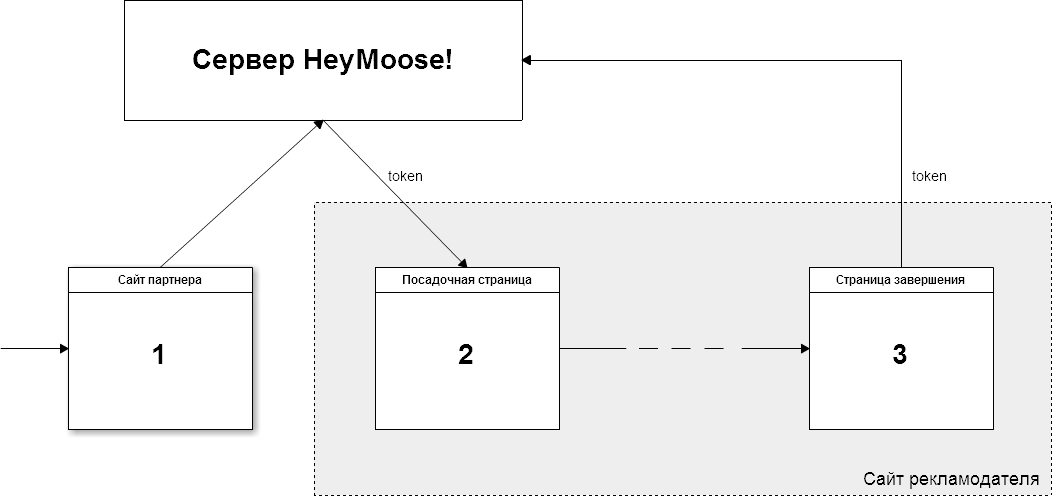
\includegraphics[width=\textwidth]{include/scheme.png}
\caption{Схема взаимодействия.}
\label{fig:scheme}
\end{figure}

\begin{enumerate}
\item Партнер размещает на \textit{рекламной площадке} (цифра \textbf{1} на схеме) описание рекламной кампании и специальную ссылку системы \heymoose. Посетитель рекламной площадки видит это описание и переходит по партнёрской ссылке.
\item Сервер \heymoose{} перенаправляет (redirect) пользователя на \textit{посадочную страницу} (цифра \textbf{2} на схеме) рекламной кампании, передавая при этом специальные GET-параметры:
	\begin{itemize}
	\item \textbf{\_hm\_token}~--- идентификатор (token) перехода в системе <<HeyMoose!>>;
	\item \textbf{\_hm\_ttl}~--- время жизни Cookie (в днях).
	\end{itemize}
\item Пользователь в процессе серфинга по сайту рекламодателя совершает \textit{действие} и попадает на \textit{страницу завершения} действия (цифра \textbf{3} на схеме). Примеры страниц завершения: страница с благодарностью за покупку; страница, следующая за страницей регистрации.
\end{enumerate}

\section{Этапы интеграции}

В этом разделе подробно описаны основные действия, которые должен совершить рекламодатель для успешной интеграции с системой \heymoose{} с использованием подтверждающего пикселя.

\subsection{Создание рекламной кампании}

Прежде всего необходимо зарегистрироваться в системе \heymoose{} в качестве рекламодателя. Для этого нужно перейти по ссылке \href{http://heymoose.com/register/advertiser/}{http://heymoose.com/register/advertiser/}, заполнить все поля в форме и нажать на кнопку <<Зарегистрироваться>>. После успешной регистрации необходимо подтвердить введенный адрес электронной почты, перейдя по ссылке в полученном письме.

Далее необходимо создать рекламную кампанию (оффер) в системе \heymoose. Для этого в личном кабинете нужно перейти в форму создания оффера, нажав на вкладку <<Создать оффер>> в разделе <<Офферы>> (рис.~\ref{fig:create-offer}).

\begin{figure}[!ht]
\centering
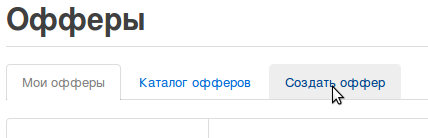
\includegraphics[width=0.5\textwidth]{include/create-offer.png}
\caption{Вкладка создания оффера.}
\label{fig:create-offer}
\end{figure}

В появившейся форме необходимо заполнить предлагаемые поля. Обязательными являются только те поля, названия которых выделены жирным шрифтом. Опишем подробнее значения каждого поля в форме создания оффера:

\begin{itemize}
\item \textbf{Название оффера}~--- название вашей рекламной кампании, которое будет отображаться партнёрам системы \heymoose. В общем случае в названием рекламной кампании может являться просто название интернет-магазина, рекламирующего товары в системе \heymoose{}, название браузерной игры и~т.п. Название оффера может иметь длину до 100 символов.
\item \textbf{Ссылка на сайт рекламодателя}~--- ссылка на главную страницу интернет-магазина (или другого сайта), которая отображается партнёрам для ознакомления с рекламируемым товаром или услугой. \textit{Данная ссылка никаким образом не участвует в процессе интеграции и предоставляется лишь для ознакомительных целей}.
\item \textbf{Партнёрская ссылка}~--- ссылка на посадочную страницу вашего сайта. Именно на этот адрес будет переходить посетитель при переходе по ссылке, размещенной партнёром на рекламной площадке. В партнёрской ссылке можно задавать GET-параметры, например, UTM-метки или другие инструменты для отслеживания источника перехода.
\item \textbf{Время жизни Cookie}~--- количество дней, которое система \heymoose{} будет отслеживать действия, совершенные пользователем, перешедшим на ваш сайт по партнёрской ссылке \heymoose.
\item \textbf{Дата запуска}~--- дата, с которой оффер будет отображаться партнёрам в каталоге рекламных предложений.
\item \textbf{Логотип}~--- небольшое изображение, характеризующее созданную рекламную кампанию, которое будет отображаться партнёрам в каталоге рекламных предложений. Принимаются изображения в формате JPG (JPEG), GIF, PNG. Максимальный размер загружаемого изображения~--- 1Мб. После загрузки изображение будет вписано в размер 150~х~100 пикселей.
\item \textbf{Действия}. Рекламная кампания может подразумевать одно или несколько завершающих действий, каждое из которых может иметь разную сумму вознаграждения для партнёра. Например, для браузерной игры рекламная кампания может иметь следующие действия: регистрация в игре, создание персонажа, прохождение второго уровня, пополнение игрового счёта. В рекламной кампании должно быть, как минимум, одно действие. Дополнительные действия можно создать, нажав на кнопку <<Добавить действие>>. Каждое действие имеет следующие поля:

	\begin{itemize}
	\item \textit{Описание}~--- краткое описание действия. Например, <<регистрация на сайте>>, <<пополнение счёта>> и~т.п.
	\item \textit{Оплата}~--- способ и сумма оплаты за действие. На данный момент в системе существует четыре способа оплаты: фиксированная плата за клик, за действие, раздельная оплата первого и последующих действий и процент с заказа или покупки. При этом \textit{вводится сумма или процент, которые оплачивает рекламодатель в общем (т.е. вознаграждение партнеру плюс комиссия системе)}.
	\item \textit{Код}~--- в общем случае это поле изменять не нужно.
	\item \textit{Время холда}~--- количество дней с момента создания действия, во время которых действие считается неподтвержденным, и рекламодатель может отменить его, если оно является невалидным или совершенным с нарушениями.
	\item \textit{Многократное прохождение}~--- будут ли отслеживаться повторные действия, совершенные пользователем, перешедшим по партнёрской ссылке.
	\end{itemize}

\item \textbf{Категории}~--- двухуровневый список тематических категорий, к которым относится рекламное предложение. Правильный выбор категорий поможет партнёрам быстрее найти ваше рекламное предложение.
\item \textbf{Регионы}~--- список регионов, с которых будет разрешен трафик на ваш сайт. Если не выбрано ни одного региона, трафик будет разрешен отовсюду. Для вашего удобства существует быстрая кнопка для выбора всех регионов СНГ.
\item \textbf{Разрешить deeplink}~--- разрешить партнёрам перенаправлять пользователей не только на указанный вами адрес, но и на другие внутренние страницы вашего сайта. Например, для интернет-магазина партнёр может перенаправлять пользователей на страницу конкретного товара. \textit{Внимание: механизм deeplink предполагает дополнительные действия по конфигурации рекламной кампании. Если вы хотите разрешить deeplink, свяжитесь с нашими менеджерами.}
\item \textbf{Краткое описание кампании}~--- текст описание, который будет отображаться в каталоге офферов. Его цель~--- вызвать у партнера заинтересованность в размещении кампании на своих рекламных площадках и уверенность в гарантированных выплатах. Постарайтесь описать здесь коротко, почему именно эта кампания будет приносить партнеру доходы. Максимальная длина текста~--- 250 символов.
\item \textbf{Подробное описание}~--- текст, в котором можно во всех подробностях описать рекламную кампанию и рассказать все то, что не поместилось в краткое описание. Чем больший текст вы разместите, тем лучше. В этом поле доступно HTML-форматирование.
\end{itemize}

После успешного создания оффера он попадет на модерацию и будет ожидать подтверждения администратором. В списке ваших рекламных кампаний вновь созданная кампания появится со статусом <<на модерации>> (рис.~\ref{fig:offer}).

\begin{figure}[!ht]
\centering
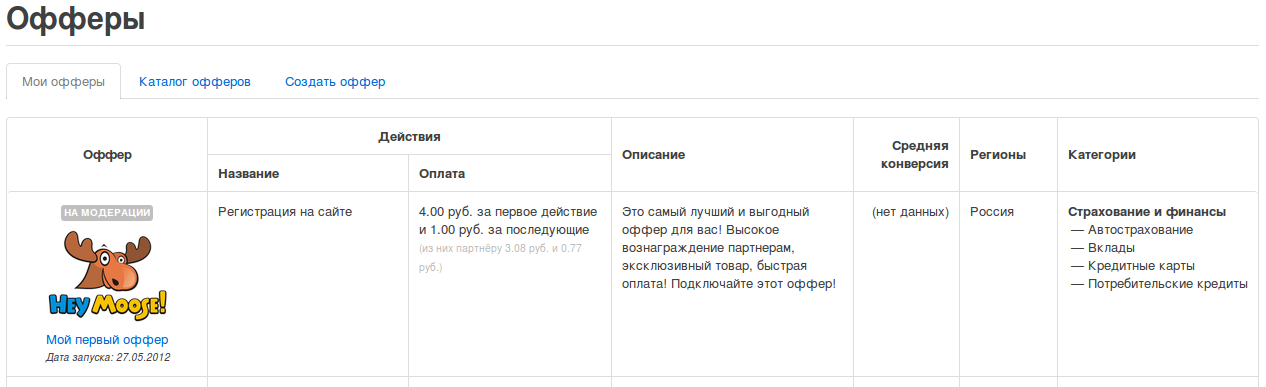
\includegraphics[width=\textwidth]{include/offer.png}
\caption{Созданная кампания в списке офферов.}
\label{fig:offer}
\end{figure}

При нажатии на логотип оффера, вы попадете на страницу описания рекламной кампании, где можете настраивать и управлять созданной рекламной кампанией.

\subsection{Пополнение счета рекламной кампании}

Для ввода наличных средств в систему \heymoose{} используется платежная система <<RoboKassa>>.

Сначала необходимо пополнить баланс рекламодателя в системе. Для этого перейдите во вкладку <<Операции со счетом>> в разделе <<Профиль>> личного кабинета. В форме пополнения счета (рис.~\ref{fig:operations}) введите необходимую сумму и нажмите кнопку <<Пополнить баланс>>. При этом вы будете перенаправлены на сайт платежной системы <<RoboKassa>>, где вам предложат проделать все необходимые действия.

\begin{figure}[!ht]
\centering
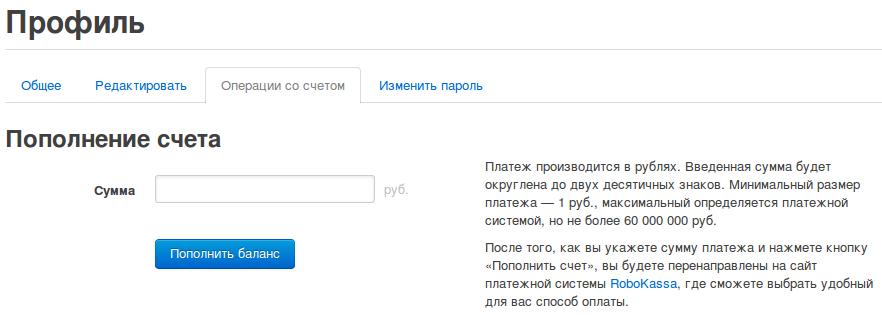
\includegraphics[width=\textwidth]{include/operations.png}
\caption{Форма пополнения счета рекламодателя.}
\label{fig:operations}
\end{figure}

После успешного пополнения счета необходимо перевести все средства или часть средств с основного баланса рекламодателя на счет созданной рекламной кампании. Для этого перейдите во вкладку <<Операции со счетом>> на странице описания рекламной кампании. В форме пополнения счета рекламной кампании (рис.~\ref{fig:offer-operations}) введите необходимую сумму и нажмите кнопку <<Пополнить счет>>.

\begin{figure}[!ht]
\centering
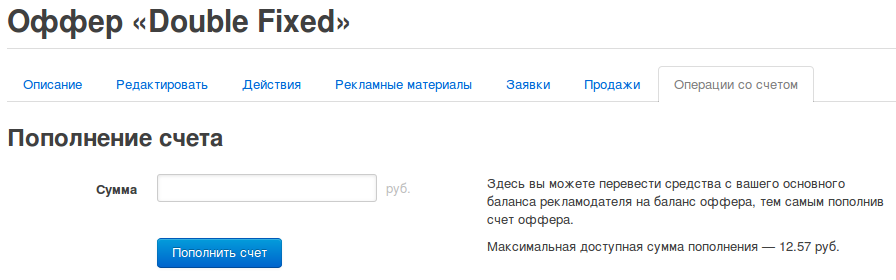
\includegraphics[width=\textwidth]{include/offer-operations.png}
\caption{Форма пополнения счета рекламной кампании.}
\label{fig:offer-operations}
\end{figure}

Теперь на счету созданной рекламной кампании есть средства для начала работы.

\subsection{Загрузка рекламных материалов}

Для того, чтобы партнеры более продуктивно рекламировали ваши товары или услуги, можно загрузить рекламные материалы в созданную кампанию. Для этого необходимо перейти во вкладку <<Рекламные материалы>> на странице с описанием рекламной кампании.

Рекламные материалы можно загрузить с помощью формы, изображенной на рис.~\ref{fig:materials}. Принимаются изображения в форматах JPG (JPEG), GIF, PNG, SWF (Flash), SVG. Максимальный размер изображения~--- 1Мб.

\begin{figure}[!ht]
\centering
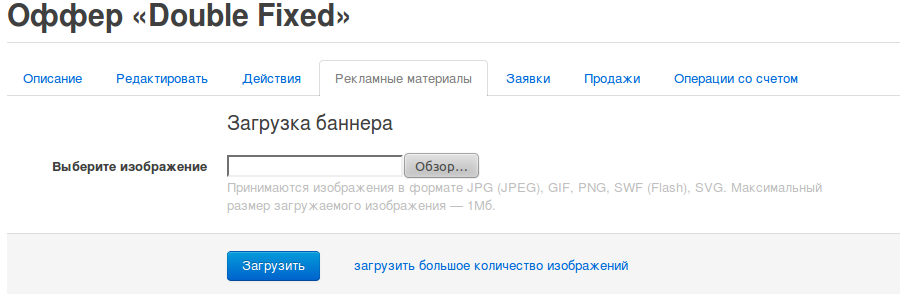
\includegraphics[width=\textwidth]{include/materials.png}
\caption{Форма загрузки рекламных материалов.}
\label{fig:materials}
\end{figure}

Для загрузки большого количества баннеров удобнее использовать форму мультизагрузки. Для этого перейдите по ссылке <<загрузить большое количество изображений>>.

\subsection{Установка подтверждающего пикселя}
\label{ssec:pixel}

Подтверждающий пиксель ставится на страницу сайта рекламодателя, означающую завершение некоторого конкретного действия пользователя (это означает, что если в при создании рекламной кампании было указано несколько действий, на разных страницах могут находиться разные подтверждающие пиксели).

Для успешной установки пикселя для рекламной кампании необходимо знать некоторую дополнительную информацию. Во-первых, это уникальный идентификатор рекламодателя в системе. Он находится в правой верхней части вашего личного кабинета рядом с вашим балансом (рис.~\ref{fig:advertiser-id}).

\begin{figure}[!ht]
\centering
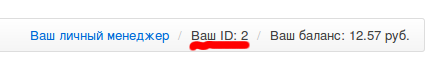
\includegraphics[width=0.7\textwidth]{include/advertiser-id.png}
\caption{Уникальный идентификатор рекламодателя.}
\label{fig:advertiser-id}
\end{figure}

Во-вторых, для каждого действия необходимо получить его уникальный код. Коды действий можно найти во вкладке <<Действия>> страницы с описанием созданной рекламной кампании (рис.~\ref{fig:suboffer-code}).

\begin{figure}[!ht]
\centering
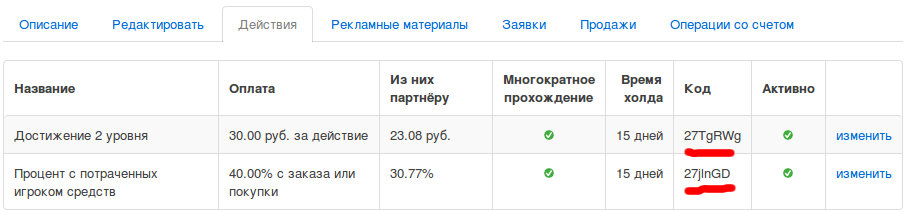
\includegraphics[width=\textwidth]{include/suboffer-code.png}
\caption{Уникальные коды действий.}
\label{fig:suboffer-code}
\end{figure}

При интеграции с использованием подтверждающего пикселя возможно несколько схем. Опишем самые распространенные из них.

\subsubsection{Выполнение одного действия с фиксированной оплатой}

Согласно этой схеме, на страницу завершения действия (внутри тега \textbf{<body></body>}) необходимо вставить следующий код (убедитесь, чтобы в значении атрибута \textbf{src} не было пробелов!):

~\\

\begin{lstlisting}[language=Pixel]
<img src="http://partner.heymoose.com/api?method=reportAction&transaction_id=TRANSACTION_ID&advertiser_id=ADVERTISER_ID&offer=OFFER_CODE" 
alt="" style="width: 0; height: 0; position: absolute;" />
\end{lstlisting}

~\\

В пикселе нужно выставлять следующие параметры:

\begin{itemize}
\item \textbf{TRANSACTION\_ID}~--- уникальный идентификатор совершенного действия (транзакции). Например, для интернет-магазина это может быть номер заказа, совершенного пользователем. Соответственно, в этом случае данный параметр должен иметь различные значения при каждом отображении пикселя. Значением параметра должна быть строка длиной менее 255 символов.
\item \textbf{ADVERTISER\_ID}~--- уникальный идентификатор рекламодателя, полученный в личном кабинете (см.~\ref{ssec:pixel}).
\item \textbf{OFFER\_CODE}~--- уникальный код действия, полученный в списке действий в описании оффера (см.~\ref{ssec:pixel}).
\end{itemize}

\subsubsection{Выполнение нескольких действий с фиксированной оплатой}
\label{sssec:fix-multiple}

Один пиксель также может <<завершать>> несколько действий одновременно. В этом случае код пикселя будет выглядеть следующим образом:

~\\

\begin{lstlisting}[language=Pixel]
<img src="http://partner.heymoose.com/api?method=reportAction&transaction_id=TRANSACTION_ID&advertiser_id=ADVERTISER_ID&offer=OFFER_CODE1,OFFER_CODE2,OFFER_CODE3" 
alt="" style="width: 0; height: 0; position: absolute;" />
\end{lstlisting}

~\\

Данный пиксель отличается от предыдущего тем, что в параметре \textbf{offer} передано несколько кодов действий, разделенных запятыми (без пробелов!). Все остальные параметры остаются такими же.

\subsubsection{Выполнение действия с процентом от совершенного заказа}

В этой схеме пиксель обычно ставится на страницу с благодарностью пользователю за совершенный заказ. Для того, чтобы система \heymoose{} смогла вычислить вознаграждение партнера и комиссию, должна быть известна общая сумма заказа. Код пикселя будет следующим:

~\\

\begin{lstlisting}[language=Pixel]
<img src="http://partner.heymoose.com/api?method=reportAction&transaction_id=TRANSACTION_ID&advertiser_id=ADVERTISER_ID&offer=OFFER_CODE:COST" 
alt="" style="width: 0; height: 0; position: absolute;" />
\end{lstlisting}

~\\

В данном пикселе параметр \textbf{offer} передается в виде \textbf{OFFER\_CODE:COST}, где \textbf{OFFER\_CODE}~--- уникальный код действия, а \textbf{COST}~--- общая сумма совершенного пользователем заказа (в рублях, разделителем рублей и копеек является точка).

Аналогично со схемой~\ref{sssec:fix-multiple}, можно передавать сразу несколько действий в формате \textbf{OFFER\_CODE1:COST1,OFFER\_CODE2:COST2,OFFER\_CODE3:COST3}.

\subsection{Запуск рекламной кампании}

После того, как вы заключили договор с \heymoose{}, настроили рекламную кампанию, загрузили необходимые материалы и установили подтверждающие пиксели, ваша рекламная кампания будет переведена в рабочее состояние. Это означает, что партнёры увидят описание кампании в каталоге офферов и смогут подать заявку на сотрудничество с рекламной кампанией.


\section{Сверка выполненных действий}

По прошествии некоторого времени после запуска рекламной кампании начнут отслеживаться действия пользователей, перешедших от партнёров сети \heymoose{}. Вы можете увидеть их в списке продаж в личном кабинете рекламодателя. Для этого перейдите во вкладку <<Продажи>> страницы описания оффера (рис.~\ref{fig:sales}).

\begin{figure}[!ht]
\centering
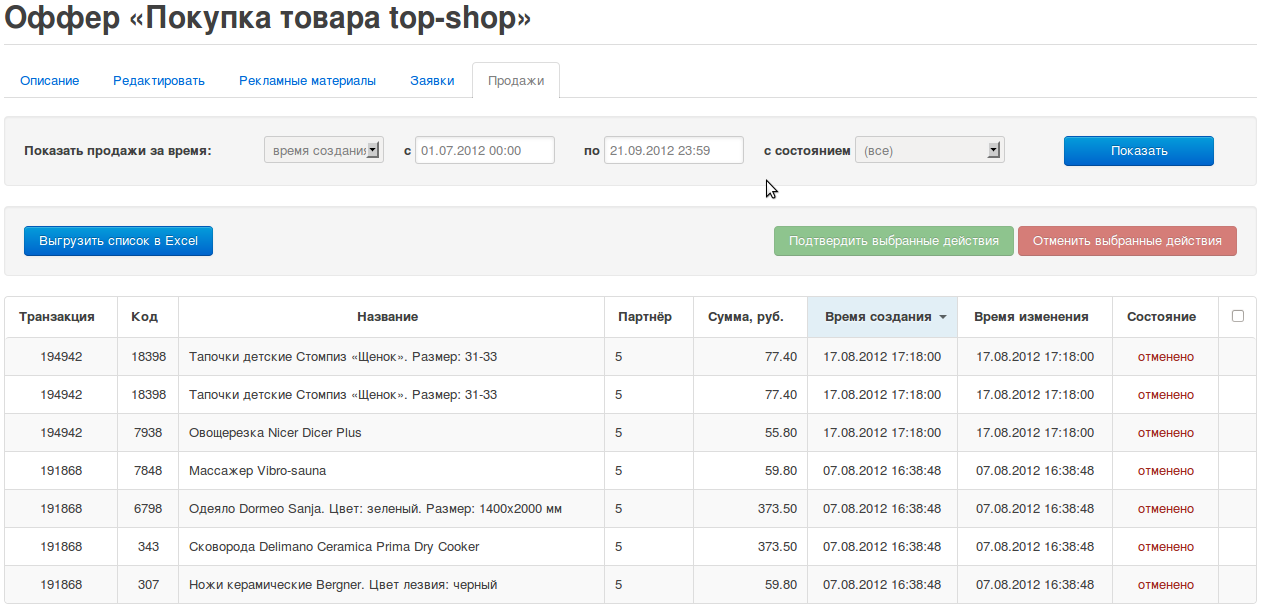
\includegraphics[width=\textwidth]{include/sales.png}
\caption{Список продаж по рекламной кампании.}
\label{fig:sales}
\end{figure}

В колонке <<Транзакция>> списка продаж находятся значения параметра \textbf{transaction\_id}, переданные в пикселе при завершении соответствующих действий. Аналогично, в колонке <<Код>> находятся значения параметра \textbf{offer}, переданные в пикселе. По этим данным можно проводить сверку списка продаж в системе \heymoose{} со внутренней статистикой вашего сайта.

Для удобства сверки существует возможность выгрузки списка продаж за определенный период в формат XLS (электронную таблицу Microsoft Excel). Выберите интересующий вас период, фильтр по состоянию и нажмите кнопку <<Показать>>. После того, как отобразится список продаж, нажмите кнопку <<Выгрузить список в Excel>>. В полученном файле будут отображены все найденные продажи.

Если при сверке оказалось, что некоторые действия являются невалидными (фейковыми), их можно отменить с помощью того же списка продаж. Для этого выберите необходимые действия с помощью флажков справа и нажмите кнопку <<Отменить выбранные действия>>. Выбранные действия получат статус <<отменено>>, а списанные за них средства вернутся на счет оффера.

Стоит подчеркнуть, что возможность отмены действий пропадает после того, как по действию заканчивается холд. Подтвержденные действия отменить также невозможно.

\section{Блокировка партнёров}

В списке продаж также можно наблюдать идентификаторы партнёров, от которых совершаются те или иные действия. Если вы заметили, что какой-то партнёр занимается накруткой трафика, использует нелегальные методы или действует подозрительно, вы можете запретить этому партнёру сотрудничать с вашей рекламной кампанией. Для этого перейдите во вкладку <<Заявки>> страницы описания оффера (рис.~\ref{fig:requests}).

\begin{figure}[!ht]
\centering
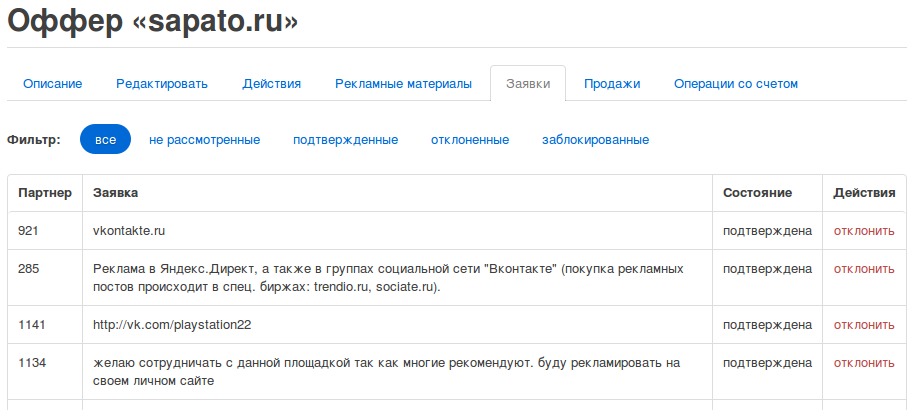
\includegraphics[width=\textwidth]{include/requests.png}
\caption{Список заявок на сотрудничество с рекламной кампанией.}
\label{fig:requests}
\end{figure}

Найдите заявку от партнёра с нужным идентификатором и нажмите кнопку <<отклонить>>. Более этот партнёр не сможет лить трафик на вашу рекламную кампанию.

Заявку можно в любой момент вернуть в прежнее состояние с помощью того же списка.

\section{Просмотр статистики}

Система \heymoose{} также предоставляет несколько срезов статистики для более удобного просмотра агрегированной информации по рекламным площадкам. Статистика обновляется в режиме реального времени.

Реализованы следующие срезы статистики:

\begin{itemize}
\item по офферам (рис.~\ref{fig:stats-offer});
\item по партнёрам (рис.~\ref{fig:stats-aff}).
\end{itemize}

\begin{figure}[!ht]
\centering
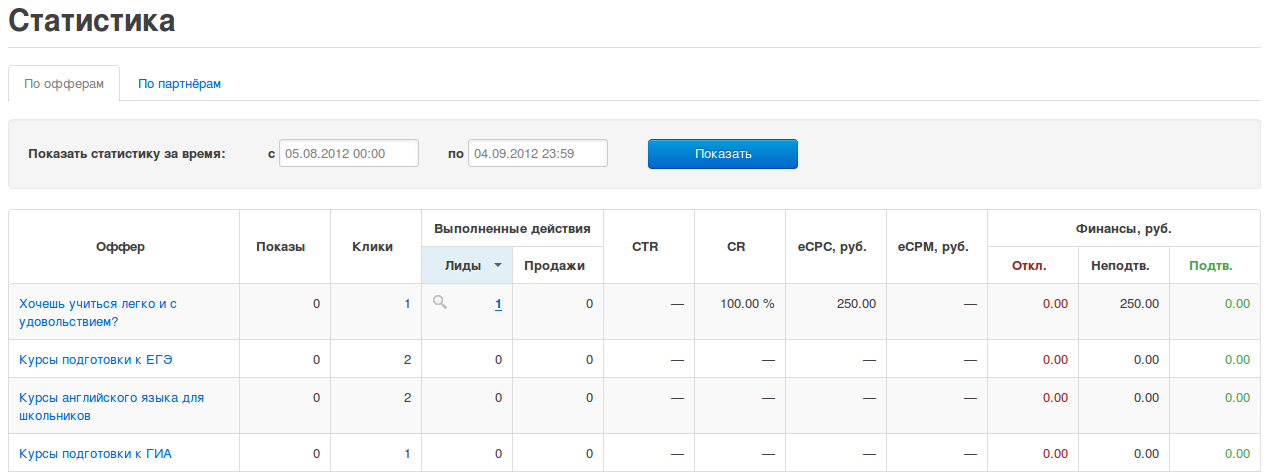
\includegraphics[width=\textwidth]{include/stats-offer.png}
\caption{Статистика по офферам.}
\label{fig:stats-offer}
\end{figure}

\begin{figure}[!ht]
\centering
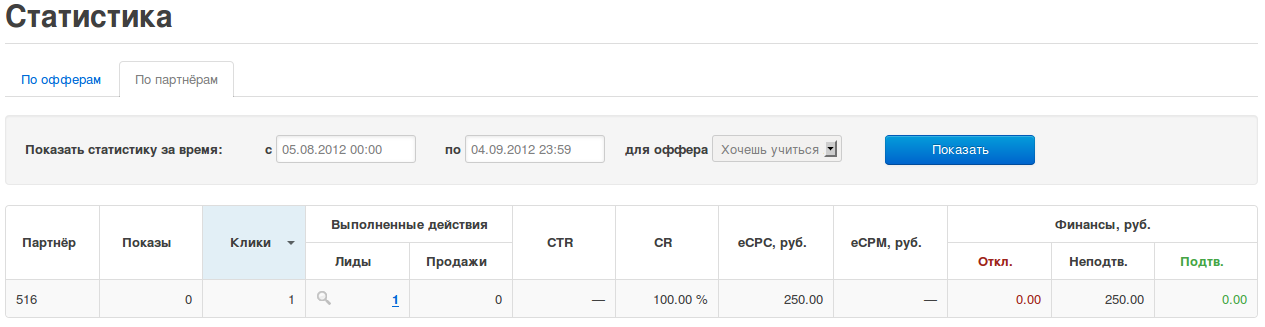
\includegraphics[width=\textwidth]{include/stats-aff.png}
\caption{Статистика по партнёрам.}
\label{fig:stats-aff}
\end{figure}

Помимо этого, кликнув на число лидов или продаж в каждой строке статистики, можно увидеть более развернутую информацию о том, какие именно действия были выполнены (рис.~\ref{fig:stats-suboffer}).

\begin{figure}[!ht]
\centering
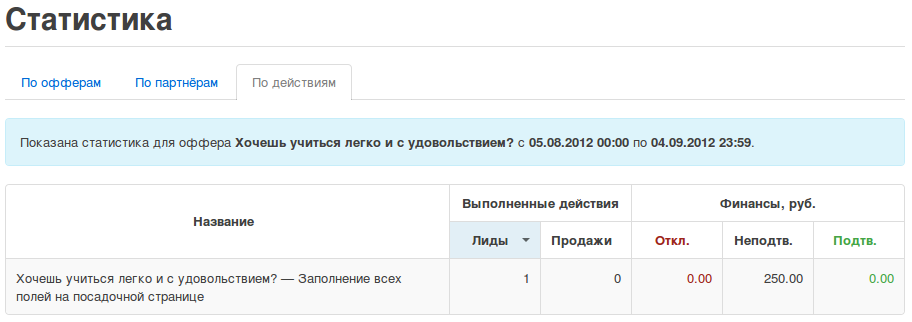
\includegraphics[width=\textwidth]{include/stats-suboffer.png}
\caption{Статистика по действиям.}
\label{fig:stats-suboffer}
\end{figure}

\end{document}
